\documentclass{article}
\usepackage[utf8]{inputenc}
\usepackage[margin=1in,includefooter]{geometry}
\usepackage{graphicx}
\usepackage{float}

\begin{document}

\begin{titlepage}
    \begin{center}
    \line(1,0){300} \\
    [0.2in]
    \huge{\bfseries Priority Queue\\ Comparison Report} \\
    \line(1,0){300} \\
    [1.5cm]
    \textsc{\LARGE Heap vs. List}\\
    [15cm]
    \end{center}
    \begin{flushright}
    \textsc{\large Samy Masadi\\
    CSCI 423\\
    March 22, 2019}
    \end{flushright}
\end{titlepage}

\tableofcontents
\thispagestyle{empty}
\cleardoublepage

\setcounter{page}{1}

\section{Summary}
This program measures the performance of priority queues using a heap structure and using a list structure. It generates several reports of time performance for each individual module for lists of several sizes. It also creates a report for a overall job scheduler using heap and list.

From the reports, we can conclude that enqueing and dequeing in a heap is O(logn) because the task of heapifying an item is divide in two. Enqueing a list is constant because it is unsorted and order does not matter. Dequeing a list is O(n) because it must search for the highest priority before removing it. For the job schedulers, the heap has better performance with O(nlogn) because it must enqueue and dequeue for all items. The list is O(n squared) because it must search all items for every item in the queue.

\newpage
\section{Methodology}
Note: Pseudocode for heap modules sourced from CSCI 423 lecture slides.
\subsection{Heap Pseudocode}
\hspace{\parindent}enQueue:

\hspace{\parindent}append(item)

\hspace{\parindent}Reheapify Sift up:

\hspace{\parindent}\hspace{\parindent}If parent is greater:

\hspace{\parindent}\hspace{\parindent}\hspace{\parindent}swap(parent, item)\\

deQueue:

\hspace{\parindent}swap(first, last)

\hspace{\parindent}pop(last)

\hspace{\parindent}Reheapify:

\hspace{\parindent}\hspace{\parindent}If child is smaller:

\hspace{\parindent}\hspace{\parindent}\hspace{\parindent}swap(child, item)

\newpage
\section{Performance Reports}
\subsection{Modules: Size 10}
\begin{table}[H]
    \begin{tabular}{c c c}
        Module & Heap & List \\ \hline
        \_init\_ & 0.000016 & 0.000002 \\ 
        enQueue & 0.000013 & 0.000004 \\
        deQueue & 0.000005 & 0.000004 \\
        sneakAPeek & 0.000001 & 0.000002 \\
        isEmpty & 0.000001 & 0.000001 \\
        size & 0.000001 & 0.000001 \\
    \end{tabular}
\end{table}

\subsection{Modules: Size 50}
\begin{table}[H]
    \begin{tabular}{c c c}
        Module & Heap & List \\ \hline
        \_init\_ & 0.000057 & 0.000002 \\ 
        enQueue & 0.000009 & 0.000003 \\
        deQueue & 0.000006 & 0.000008 \\
        sneakAPeek & 0.000001 & 0.000007 \\
        isEmpty & 0.000001 & 0.000001 \\
        size & 0.000000 & 0.000000 \\
    \end{tabular}
\end{table}

\subsection{Modules: Size 500}
\begin{table}[H]
    \begin{tabular}{c c c}
        Module & Heap & List \\ \hline
        \_init\_ & 0.000590 & 0.000003 \\ 
        enQueue & 0.000009 & 0.000003 \\
        deQueue & 0.000009 & 0.000058 \\
        sneakAPeek & 0.000001 & 0.000058 \\
        isEmpty & 0.000001 & 0.000001 \\
        size & 0.000001 & 0.000000 \\
    \end{tabular}
\end{table}

\subsection{Modules: Size 1000}
\begin{table}[H]
    \begin{tabular}{c c c}
        Module & Heap & List \\ \hline
        \_init\_ & 0.001177 & 0.000004 \\ 
        enQueue & 0.000009 & 0.000004 \\
        deQueue & 0.000011 & 0.000146 \\
        sneakAPeek & 0.000001 & 0.000139 \\
        isEmpty & 0.000001 & 0.000001 \\
        size & 0.000000 & 0.000000 \\
    \end{tabular}
\end{table}

\subsection{Modules: Size 5000}
\begin{table}[H]
    \begin{tabular}{c c c}
        Module & Heap & List \\ \hline
        \_init\_ & 0.005858 & 0.000008 \\ 
        enQueue & 0.000009 & 0.000003 \\
        deQueue & 0.000012 & 0.000658 \\
        sneakAPeek & 0.000001 & 0.000657 \\
        isEmpty & 0.000001 & 0.000001 \\
        size & 0.000001 & 0.000001 \\
    \end{tabular}
\end{table}

\subsection{Modules: Size 10000}
\begin{table}[H]
    \begin{tabular}{c c c}
        Module & Heap & List \\ \hline
        \_init\_ & 0.012278 & 0.000052 \\ 
        enQueue & 0.000010 & 0.000033 \\
        deQueue & 0.000014 & 0.001183 \\
        sneakAPeek & 0.000001 & 0.001175 \\
        isEmpty & 0.000001 & 0.000001 \\
        size & 0.000000 & 0.000000 \\
    \end{tabular}
\end{table}

\subsection{Modules: Size 50000}
\begin{table}[H]
    \begin{tabular}{c c c}
        Module & Heap & List \\ \hline
        \_init\_ & 0.058573 & 0.000193 \\ 
        enQueue & 0.000010 & 0.000006 \\
        deQueue & 0.000018 & 0.005876 \\
        sneakAPeek & 0.000001 & 0.006060 \\
        isEmpty & 0.000001 & 0.000001 \\
        size & 0.000001 & 0.000001 \\
    \end{tabular}
\end{table}

\subsection{Job Scheduler Test Results}
\begin{table}[H]
    \begin{tabular}{c c c}
        Size & Heap & List \\ \hline
        10 & 0.002792 & 0.000860 \\ 
        50 & 0.003096 & 0.001290 \\
        500 & 0.007834 & 0.031011 \\
        1000 & 0.013855 & 0.119394 \\
        5000 & 0.069740 & 2.958742 \\
        10000 & 0.144353 & 11.856617 \\
        50000 & 0.817438 & 297.10306
    \end{tabular}
\end{table}

\newpage
\section{Complexity Analysis}
\subsection{Time Efficiency}
\begin{table}[H]
    \begin{tabular}{c c c}
        Module & Heap & List \\ \hline
        \_init\_ & O(nlogn) & O(n) \\ 
        enQueue & O(logn) & O(1) \\
        deQueue & O(logn) & O(n) \\
        sneakAPeek & O(1) & O(n) \\
        isEmpty & O(1) & O(1) \\
        size & O(1) & O(1) \\
        scheduler & O(nlogn) & O(n^2)
    \end{tabular}
\end{table}

\newpage
\section{Schedule}
March 3: Begin work on PQ\_Heap: \_init\_; enQueue; deQueue

Completed: none\\
March 10: Finish PQ\_Heap; start PQ\_List: \_init\_: enQueue; deQueue

Completed: none\\
March 17: Finish PQ\_List; Conduct time trials; Begin Report

Completed: none\\
March 22: Complete Report

Completed: PQ\_Heap, PQ\_List, Conducted time trials

Report completed March 24

\newpage
\section{Screenshot Showcase}
\begin{figure}[H]
    \centering
    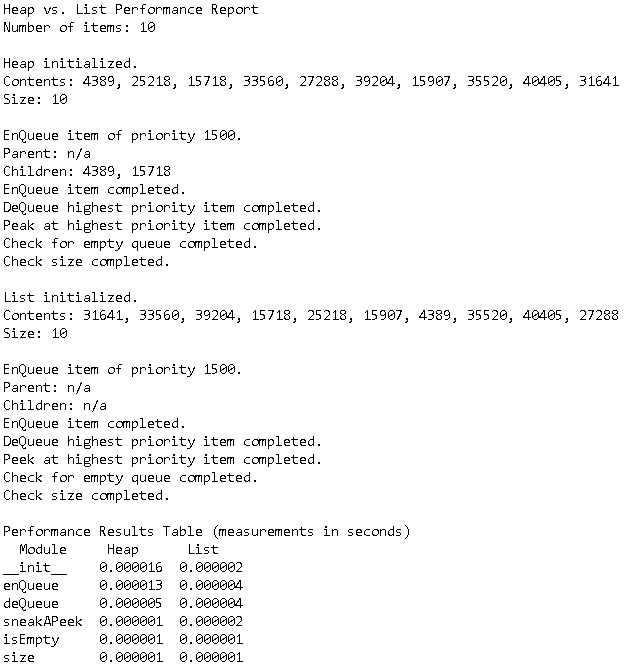
\includegraphics{report10.PNG}
    \caption{report10.txt: Output report for 10 items}
\end{figure}
\begin{figure}[H]
    \centering
    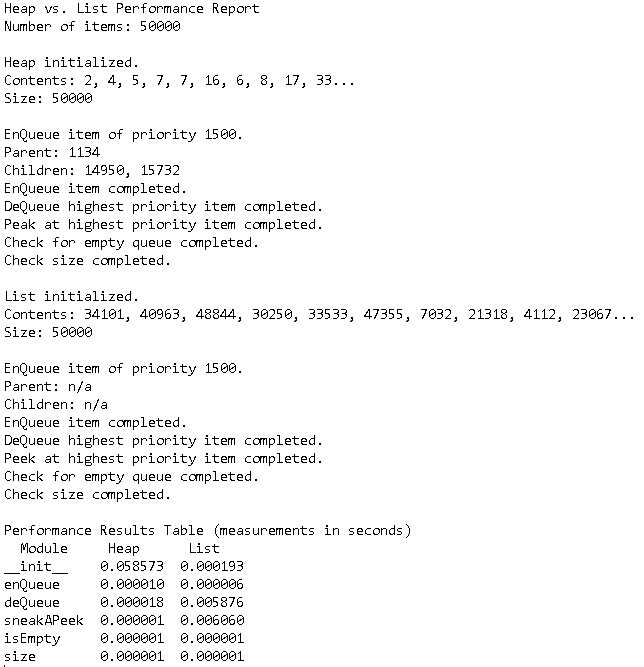
\includegraphics{report50000.PNG}
    \caption{report50000.txt: Output report for 50000 items}
\end{figure}
\begin{figure}[H]
    \centering
    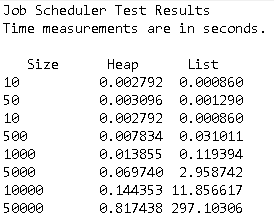
\includegraphics{scheduler_results.PNG}
    \caption{scheduler\_results.txt output file}
\end{figure}

\end{document}
